\documentclass[12pt]{article}
\usepackage{tikz}
\usepackage{wrapfig}
\pagestyle{empty}
\textwidth      165mm
\textheight     250mm
\topmargin      -16mm
\oddsidemargin  -2mm
\evensidemargin -2mm

\newcommand{\set}[1]{\left\{
    \begin{array}{l}#1
    \end{array}
  \right\}}

\newcommand{\sset}[2]{\left\{~#1 \left|
      \begin{array}{l}#2\end{array}
    \right.     \right\}}

\newcommand{\id}[1]{\mbox{\textit{#1}}}
\newcommand{\tuple}[1]{\langle #1 \rangle}
\newcommand{\impl}{\mathbin{\Rightarrow}}
\newcommand{\biim}{\mathbin{\Leftrightarrow}}

\begin{document}

\begin{center}
{\sc The University of Melbourne
\\
School of Computing and Information Systems
\\ 
COMP30026 Models of Computation}
\bigskip \\
{\Large\bf Assignment 1, 2017}
\bigskip \\
{\large Released: 11 August.  Deadline: 1 September at 23:00}
\end{center}

\section*{Purpose}
To improve your understanding of propositional and first-order 
predicate logic, including their use in mechanized reasoning.
To develop skills in analysis and formal reasoning about
complex concepts, and to practise writing down formal arguments.

\section*{Five challenges}

\subsection*{Challenge 1}
On the Island of Knights and Knaves, everyone is a knight or knave.
Knights always tell the truth.
Knaves always lie.
You meet three people, let us call them A, B and C.
A says to you:
``If I am a knight then my two friends here are knaves.''
Use propositional logic to determine whether this statement
gives you any real information.
What, if anything, can be deduced about A, B, and C?

\subsection*{Challenge 2}
Let $\varphi$ and $\psi$ be these propositional formulas:
\begin{itemize}
\item
$\varphi : ((P \impl S) \land (Q \impl R) \land (R \impl P)) \impl S$.
\item
$\psi : (((P \lor Q) \impl S) \land (\neg P \impl (R \impl Q)) \land (R \lor S)) \impl S$.
\end{itemize}
\begin{enumerate}
\item
Negate $\varphi$ and transform the resulting formula to CNF.
\item
\emph{Either} use resolution on the resulting set of clauses and prove
that $\varphi$ is valid by deriving $\bot$, \emph{or} show that
$\varphi$ is in fact non-valid.
\item
Negate $\psi$ and transform the resulting formula to CNF.
\item
\emph{Either} use resolution on the resulting set of clauses and prove
that $\psi$ is valid by deriving $\bot$, \emph{or} show that $\psi$ is
in fact non-valid.
\end{enumerate}

\subsection*{Challenge 3}
Show that the closed formula
\[
  \left[ \forall x \forall y (P(x,y) \impl P(h(x),h(h(y)))) \right]
        \quad \impl \quad \forall x (P(x,h(x)) \land P(h(h(x)),x))
\]
is non-valid but satisfiable.

\subsection*{Challenge 4}
For this question use the following predicates:
\begin{itemize}
\item
$S(x)$, which stands for ``$x$ is a surgeon''
\item
$P(x,y)$, which stands for ``$x$ is a patient of $y$''
\item
$R(x)$, which stands for ``$x$ recovers''
\item
$H(x)$, which stands for ``$x$ is happy''
\end{itemize}
\begin{enumerate}
\item
Express, \emph{as a formula in first-order predicate logic}
(not clausal form), this statement $S_1$:
``A surgeon with no patients is happy.''
(Be careful to get this right; most of the following depends
on this.)
\item
Express, \emph{as a formula in first-order predicate logic}
(not clausal form), this statement $S_2$:
``A surgeon is happy if all her patients recover.''
(Be even more careful here.)
\item
Translate $S_2$ to clausal form (remaining careful).
\item
Translate \emph{the negation of} $S_1$ to clausal form
(still taking care.)
\item
Give a proof by resolution to show that $S_1$ follows from $S_2$.
\end{enumerate}

\subsection*{Challenge 5}
\begin{wrapfigure}[12]{r}{.2\textwidth}
\begin{center}
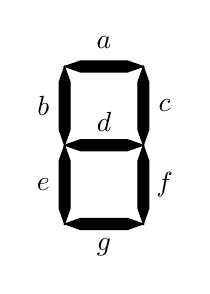
\begin{tikzpicture}
\begin{scope}[scale=0.1]

\path[draw,fill]%
(-5,1)--(-3,1.7)--(3,1.7)--(5,1)--(3,0.3)--(-3,0.3)--cycle;
\path[draw,fill]%
(-5,11)--(-3,11.7)--(3,11.7)--(5,11)--(3,10.3)--(-3,10.3)--cycle;
\path[draw,fill]%
(-5,21)--(-3,21.7)--(3,21.7)--(5,21)--(3,20.3)--(-3,20.3)--cycle;
\path[draw,fill]%
(5,1)--(4.3,3)--(4.3,9)--(5,11)--(5.7,9)--(5.7,3)--cycle;
\path[draw,fill]%
(5,11)--(4.3,13)--(4.3,19)--(5,21)--(5.7,19)--(5.7,13)--cycle;
\path[draw,fill]%
(-5,11)--(-4.3,13)--(-4.3,19)--(-5,21)--(-5.7,19)--(-5.7,13)--cycle;
\path[draw,fill]%
(-5,1)--(-4.3,3)--(-4.3,9)--(-5,11)--(-5.7,9)--(-5.7,3)--cycle;

\node at (-7.7,16) {$b$};
\node at (-7.7,6)  {$e$};
\node at (0,24)    {$a$};
\node at (0,14)    {$d$};
\node at (0,-2)    {$g$};
\node at (7.7,16)  {$c$};
\node at (7.7,6)   {$f$};

\end{scope}
\end{tikzpicture}
\end{center}
\end{wrapfigure}
Consider a single-digit display able to show the eight digits 0--7.
The display has seven LEDs (labelled $a$--$g$),
as shown on the right.
For example, to display the digit 3, all segments except
$b$ and $e$ should light up.
Each of the seven segments a--g can be considered a propositional
function of three propositional variables $X$, $Y$ and $Z$, with
input $XYZ$ specifying the desired digit in binary notation.
For example, for input $XYZ = 011$ (that is, $X$ being false and
$Y$ and $Z$ being true) the outputs $b$ and $e$ should be 0
(False) while the rest should be 1 (True).
In fact, the truth tables for all the functions $a$--$g$ are as
follows:
\[
\begin{array}{ccc|ccccccc}
   X & Y & Z & a & b & c & d & e & f & g
\\ \hline
   0 & 0 & 0 & 1 & 1 & 1 & 0 & 1 & 1 & 1
\\ 0 & 0 & 1 & 0 & 0 & 1 & 0 & 0 & 1 & 0
\\ 0 & 1 & 0 & 1 & 0 & 1 & 1 & 1 & 0 & 1
\\ 0 & 1 & 1 & 1 & 0 & 1 & 1 & 0 & 1 & 1
\\ 1 & 0 & 0 & 0 & 1 & 1 & 1 & 0 & 1 & 0
\\ 1 & 0 & 1 & 1 & 1 & 0 & 1 & 0 & 1 & 1
\\ 1 & 1 & 0 & 1 & 1 & 0 & 1 & 1 & 1 & 1
\\ 1 & 1 & 1 & 1 & 0 & 1 & 0 & 0 & 1 & 0
\end{array}
\]
The single-digit display must be implemented with logic circuitry.
Here we assume that only three types of logic gates are available.
An \emph{and-gate} takes two inputs and produces, as output, the
conjunction ($\land$) of the inputs.
Similarly, an \emph{or-gate} implements disjunction ($\lor$).
Finally, an \emph{inverter} takes a single input and negates it.

The task here is to design a circuit for all of $a$--$g$ using as
few gates as possible.
We can specify the circuit by writing down the Boolean equations
for each of the outputs $a$--$g$.
For example, we can define $f = X \lor \neg Y \lor Z$, which shows
that $f$ can be implemented with three gates.
Since we want to use as few gates as possible, it is important to
look for cases where outputs can be \emph{shared}, or reused.
For example, if we already have implemented $b$ then we could
define $f = b \lor Z$, using just one gate.
Note that any sub-circuit that you want to share (that is, you
want to direct its output to different places), the output must
have a name.
You can define as many ``helper'' functions as you please, to
create the smallest possible solution.

The answer to this question must be submitted separately on Grok
(details below).
You are to submit a text file consisting of one line per
definition (so not Haskell code; this is not a Haskell programming 
exercise).
This file will be tested automatically, so it is important that
you follow the notational conventions exactly.
We write $\neg$ as \texttt{-} and $\lor$ as \texttt{+}.
We write $\land$ as \texttt{.}, or, simpler, we just leave it out,
so that concatenation of expressions denotes their conjunction.
Here is an example set of equations (for a different problem):
\begin{verbatim}
    # An example of a set of equations in the correct format:

    a = -Y Z + Y -Z + X -Y -Z
    b = u + X (Y + Z)
    c = X + -(Y Z)
    d = u + X a
    u = -X -Y
    # u is an auxiliary function introduced to simplify b and d
\end{verbatim}
Empty lines, and lines that start with `\#', are ignored.
Input variables are in upper case.
Negation binds tighter than conjunction, which in
turn binds tighter than disjunction.
So the equation for $a$ says that
$a = (\neg Y \land Z) \lor (Y \land \neg Z) \lor (X \land \neg Y \land \neg Z)$.
Note the use of a helper function $u$, allowing $b$ and $d$ to
share some circuitry.
Also note that we do not allow any feedback loops in the circuit.
In the example above, $d$ depends on $a$, so $a$ is not allowed
to depend, directly or indirectly, on $d$ (and indeed it does not).

\section*{Submission and assessment}
Some of the problems are harder than others.
All should be solved and submitted by students individually.
Your solution will count for 10 marks out of 100 for the subject.
Each question is worth 2~marks.
Marks are primarily allocated for correctness, but elegance and how
clearly you communicate your thinking will also be taken into account.
For Challenge 5, there will be 1 mark for a correct solution. 
After that, your mark depends on which quartile your solution sits in, 
when we order all solutions by increasing number of gates.
If it falls in the best quartile (that is, within the 25\% of
solutions that use the fewest gates), we add 1 mark.
If you are in the next quartile, we add 0.5 marks.
Otherwise no marks are added to the mark for correctness.

The deadline is 1 September at 23:00.
Late submission will be possible, but a late submission penalty will
apply: a flagfall of 2 marks, and then 1 mark per 12 hours late.

For the first four challenges, submit a PDF document via the LMS.
This document should be no more than 1 MB in size.
If you produce an MS Word document, it must be exported
and submitted as PDF, and satisfy the space limit of 1 MB.
We also accept \emph{neat} hand-written submissions, but these must be
scanned and provided as PDF, and again, they must respect the size limit.
If you scan your document, make sure you set the resolution so that
the generated document is no more than 1 MB.

Being neat is easier if you type-set your answers, but not all
typesetting software does a good job of presenting mathematical formulas.
The best tool for this is \LaTeX, which is worth learning if you expect
that you will later have to produce large technical documents.
Admittedly, diagrams are tedious to do with \LaTeX,
even when using sophisticated packages such as Tikz.
You could, of course, mix typeset text with hand-drawn diagrams.
In case you want to use the assignment to get some \LaTeX\ practice,
I will leave the source for this document in the
content area where you find the PDF version.

For challenge 5, submit a text file on Grok.
You will receive immediate feedback from an elementary test,
which checks that your input has the correct format, and that it implements
the desired circuit correctly.
Note that on Grok, ``saving'' your file does not mean submitting it
for marking. 
To submit, you need to click ``mark''.
You can submit as many times as you like.
What gets marked is the last submission you have made before the deadline.

Make sure that you have enough time towards the end of the assignment
to present your solutions carefully.
A nice presentation is sometimes more time consuming than solving the
problems.
Start early; note that time you put in early usually turns out more
productive than a last-minute effort.
For Challenge 5 in particular, you don't want to submit ``improved''
solutions a few minutes before the deadline, as they may turn out
to be wrong and you wont' have time to fix this.

Individual work is expected, but if you get stuck, email Matt or Harald
a precise description of the problem, bring up the problem at the
lecture, or (our preferred option) use the LMS discussion board.
The COMP30026 LMS discussion forum is both useful and appropriate
for this;
soliciting help from sources other than the above
will be considered cheating and will lead to disciplinary action.

\begin{flushright}
Harald S{\o}ndergaard
\\ 7 August 2017
\end{flushright}

\end{document}
